
\chapter{Einleitung}
    \section{Motivation}
    Schach ist ein traditionsreiches und abwechslungsreiches Brettspiel, deren Ursprung nicht genau bestimmt werden kann. Es wird vermutet, dass das erste schachähnliche Spiel  \textit{Tschaturanga} seinen Ursprung in Nordindien um 600 n. Chr. hatte \cite{schachgeschichte}.
    Im Laufe der Jahrhunderte hat Schach eine bedeutende Rolle in der Kultur und Geschichte gespielt. So wurde beispielsweise die Schach-WM 1972 eine Art Machtkampf im kalten Krieg zwischen der UdSSR, welche den damaligen Schach dominierten, und der USA\footnote{Quelle: \url{https://www.geo.de/magazine/geo-epoche/19054-rtkl-schachweltmeisterschaft-wie-ein-schachspiel-zum-wettstreit-der} am 22. April 2023}.
    Schach bleibt bis heute ein beliebtes Spiel, welches 2020 durch die Netflix Serie \textit{Damengambit} und 2022 durch den Betrugsvorwurf von Magnus Carlsen an seinen 19-jährigen Gegner Hans Niemann\footnote{Quelle: \url{https://www.sportschau.de/schach/magnus-carlsen-hans-niemann-ermittlungen-100.html} am 22. April 2023} eine breitere Aufmerksamkeit erhielt (siehe Abbildung \ref{fig:Schachinteresse}). 
    
    \begin{figure}[ht]
\raggedleft
  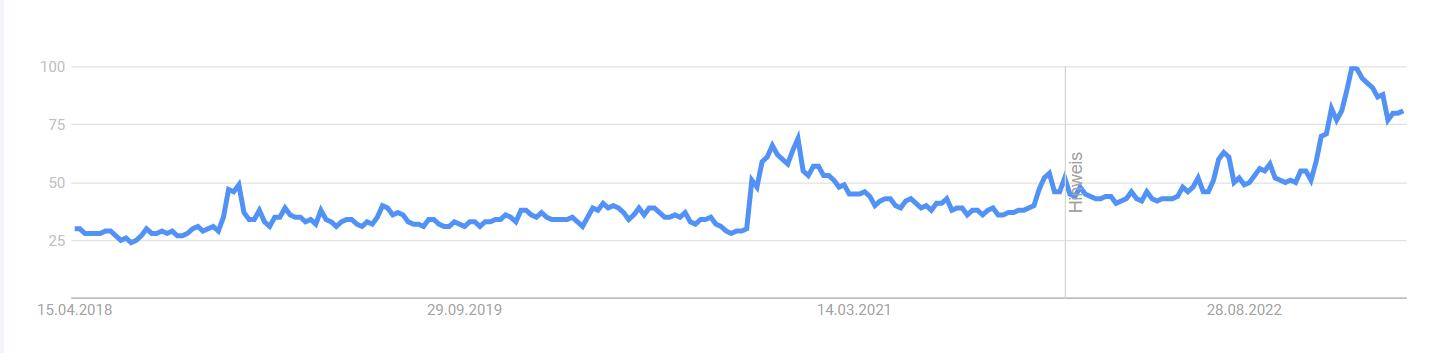
\includegraphics[width=\textwidth]{Schachentwicklung.jpg}
    \footnotesize\sffamily\textbf{Quelle:} \url{https://trends.google.de/}
  \caption{Relatives Suchinteresse des Wortes \textit{Chess} auf Google in den letzten 5 Jahren.}
  \label{fig:Schachinteresse}
\end{figure}

     Darüber hinaus hat Schach im digitalen Zeitalter eine neue Popularität erreicht. Online-Schachplattformen wie \url{chess.com} verzeichnen Milliarden von Live-Partien\footnote{Quelle: \url{https://www.chess.com/forum/view/general/weve-reached-3000000000-live-chess-games} am 22. April 2023}, während Schach Live-Streams auf Plattformen wie \url{twitch.com} Millionen von Followern anziehen\footnote{Quelle: \url{https://www.twitch.tv/chess} am 27. April 2023}.
     
Die Entwicklung einer webbasierten Multiplayer-Schach-App bietet eine einzigartige Gelegenheit, ein traditionsreiches und beliebtes Spiel im digitalen Zeitalter weiter zu entwickeln. Meine Motivation für diese Arbeit besteht darin, eine App zu entwickeln, die die Grundlagen einer Schach-App enthält und gleichzeitig eine solide Basis für zukünftige Erweiterungen und Verbesserungen bietet. Insbesondere plane ich in Zukunft, innovative Funktionen zu integrieren, die bislang in den gängigen Schach-Apps nicht vorhanden sind, wie z.B. die Möglichkeit, unterschiedliche Schachfiguren und -bretter als Belohnungen freizuschalten oder mit Freunden eine Gruppe zu gründen, welche in einer Liga auf- und absteigen kann. Durch die Entwicklung einer Schach-App mit neuen Funktionalitäten kann ich dazu beitragen, die Popularität von Schach zu steigern und vor allem das Spiel einem breiteren Publikum zugänglich zu machen.
    \section{Zielsetzung}
    Diese Bachelorarbeit hat das Ziel eine Schach-App zu entwerfen und zu implementieren, die eine intuitive User Experience und ein ansprechendes User Interface mit vielen nützlichen Funktionen beinhaltet.
    
    User Experience (kurz UX) bezieht sich darauf wie ein Nutzer sich auf einer Anwendung bewegt und wie einfach und angenehm es für den Nutzer ist, die Funktionen der Anwendung zu verwenden.
    
    Das User Interface (kurz UI) beschäftigt sich mit der visuellen und interaktiven Gestaltung von Benutzeroberflächen. Es umfasst die Gestaltung von Buttons, Formularen und anderen visuellen Komponenten, sowie das Feedback dieser Komponenten, wie zum Beispiel die Rückmeldung einer fehlgeschlagenen Anmeldung.
    Zusammengefasst beschäftigt sich UX damit, wie man eine Anwendung verwendet und UI damit, wie die Benutzeroberfläche der Anwendung aussieht.\cite{webdesign}
        
        Funktionen der Schach-App sind unter anderem das Registrieren und Anmelden, das Versenden, Annehmen und Ablehnen von Freundschaftsanfragen, das Zuschauen bei laufenden Spielen, das Herausfordern von Freunden zu Schachspielen und natürlich das Spielen von Schachpartien mit einem Chat und verschiedenen Einstellungsmöglichkeiten der Schach Uhren selbst.
    Dabei wird besonderer Wert auf die Verwendung moderner Web-Technologien wie React, Node.js, Socket.IO, Redis und PostgeSQL gelegt, um eine optimale Benutzererfahrung und Skalierbarkeit zu gewährleisten. Darüber hinaus soll die Arbeit einen Überblick über die technischen Herausforderungen und Lösungen im Zusammenhang mit der Implementierung einer solchen Schach-App bieten.
    
    \section{Aufbau der Arbeit}
Diese Bachelorarbeit gliedert sich in sechs Hauptkapitel, die jeweils unterschiedliche Aspekte der Entwicklung und Implementierung der Schach-App behandeln.

Im ersten Kapitel, der \textit{Einleitung}, werden die Motivation für die Entwicklung der Schach-App, die Zielsetzung der Arbeit und der Aufbau der Arbeit selbst vorgestellt.

Das zweite Kapitel, \textit{Theoretische Grundlagen}, erläutert die Grundlagen von Schach als Spiel sowie die verwendeten Web-Technologien wie Node.js, Express, Socket.io, React und PostgreSQL, die für das Verständnis der nachfolgenden Kapitel wichtig sind.

Im dritten Kapitel, \textit{Systemarchitektur}, wird die Gesamtarchitektur der Schach-App beschrieben, einschließlich der Unterteilung in Frontend und Backend, der Datenbankstruktur und der Kommunikation zwischen den verschiedenen Komponenten.

Das vierte Kapitel, \textit{Implementierung}, geht auf die praktische Umsetzung der Schach-App ein, indem es die Entwicklungsprozesse für das Frontend und das Backend sowie die Integration der Datenbanken erläutert.

Das fünfte Kapitel, \textit{Tests und Evaluation}, behandelt die verschiedenen Tests, die durchgeführt wurden, um die Funktionalität, Usability, Performance und Sicherheit der Schach-App zu bewerten.

Im abschließenden sechsten Kapitel, \textit{Fazit und Ausblick}, werden die Ergebnisse der Arbeit zusammengefasst, eventuelle Limitationen diskutiert und mögliche Erweiterungen und Weiterentwicklungen für die Schach-App vorgeschlagen.

Die Arbeit endet mit dem \textit{Anhang}, der zusätzliche Grafiken und die Liste der verwendeten Literatur enthält.